% This must be in the first 5 lines to tell arXiv to use pdfLaTeX, which is strongly recommended.
\pdfoutput=1
% In particular, the hyperref package requires pdfLaTeX in order to break URLs across lines.

\documentclass[11pt]{article}

% Remove the "review" option to generate the final version.
\usepackage[review]{ACL2023}

% Standard package includes
\usepackage{times}
\usepackage{latexsym}

% For proper rendering and hyphenation of words containing Latin characters
% (including in bib files)
\usepackage[T1]{fontenc}
% For Vietnamese characters
% \usepackage[T5]{fontenc}
% See https://www.latex-project.org/help/documentation/encguide.pdf for other
% character sets

% This assumes your files are encoded as UTF8
\usepackage[utf8]{inputenc}

% This is not strictly necessary, and may be commented out.
% However, it will improve the layout of the manuscript,
% and will typically save some space.
\usepackage{microtype}

% This is also not strictly necessary, and may be commented out.
% However, it will improve the aesthetics of text in
% the typewriter font.
\usepackage{inconsolata}
\usepackage{graphicx}

% If the title and author information does not fit in the area allocated,
% uncomment the following
%
%\setlength\titlebox{<dim>}
%
% and set <dim> to something 5cm or larger.

% Tables
\usepackage{booktabs}
\usepackage{multirow}

% Urls
\usepackage{hyperref}

% For naming embeddings
\newcommand{\Embed}[1]{\texttt{#1}}

% For naming classifiers
\newcommand{\Cls}[1]{\texttt{#1}}

% For naming transformations
\newcommand{\Trans}[1]{\textsl{`#1'}}

\title{Semantic information inside sentence embeddings}

\author{Leixin Zhang \\ 
    Computational Linguistics\\
    Seminar für Sprachwissenschaft,
    Universität Tübingen, Germany \\ 
    \texttt{leixin.zhang@student.uni-tuebingen.de}
    }
\author{David Burian\\
  Charles University, Prague\\
  \texttt{david.burian@matfyz.cz}
  }
 \author{Vojtěch John\\
 Charles University, Prague\\
 }
  % Second Author \\
  % Affiliation / Address line 1 \\
  % Affiliation / Address line 2 \\
  % Affiliation / Address line 3 \\
  % \texttt{email@domain} \\}

\begin{document}
\maketitle

\begin{abstract}
This is abstract
\end{abstract}

\section{Introduction}

\section{Related work}

% Costra corpus
Costra corpus~\cite{baranvcikova2020costra}

% SBERT
SBERT~\cite{reimers2019sentence}

% Doc2vec
Doc2vec~\cite{le2014distributed}


\section{Experiments}

\subsection{Costra corpus}

% Deep dive into the properties of the datsaet
%   - transformation terminology = transformation
%   - contextualized and distance vector to relation vector
%   - types and explanations of transformations
%   - dataset statistics (count of seeds, sentences in total, transformation
%   distributions)

We define \emph{relation vector} as the ....
To per
Costra 

\subsection{Embeddings}\label{sec:embeddings}

% List the embeddings we are going to work with. Focus only on the core ones,
% which are used often throughout the tasks.
We focus mainly on two sets of embeddings: \Embed{doc2vec} predicted by Doc2vec
model trained on 1M of Czech sentences and \Embed{sbert} predicted by
pretrained SBERT multilingual model. Additionally we also experimented with
supervised method using the same SBERT model --- we call this embedding
\Embed{sbert\_supervised}.

% David: I would maybe skip the part about training shorter embeddings. But
% that can wait for the paper submit.
For training the Doc2vec model, we have used the implementation of Doc2vec
algorithm available in the Python package gensim, using a window of size 4 and
considering every word that occured at all (no pruning of rare words) and the
vector size of 512. We have also tried training Doc2Vec models with different
embedding sizes (2, 3, 10, 100, 256), partly so that we could see, ehat impact
the size change has on the semantic label predictability, partly (especially if
we detected a positive correlation between the embedding size and the semantic
label predictability) in order to try and get hint as to how prominent the
specific semantic features are (i.e. which is the smallest vector size at which
given semantic label is predictable from the corresponding embeddings).


To obtain \Embed{sbert\_supervised} we splitted the corpus into 5 folds. For
each fold, the model trained on the remaining 4 folds and produced embeddings
for the one remaining fold. This gave us 5 sets of disjunct embeddings, each
trained on slightly different data. For training we used softmax loss, which
classifies sentence and its corresponding seed sentence into the set of all
possible transformations. This gives the model incentive to produce embeddings
that are easily distinguishable for different transformations.


\subsection{Tasks}




% High overview of the tasks that were carried out as well as some motivation for
% doing them. Give the reader a quick overview of the work we've done.



In addition to visualizing the embeddings of derivation sentences, we employ
several approaches to test whether our trained sentence embeddings can
accurately characterize the derivation sentence types.

\subsubsection{Visualization}



\subsubsection{Cosine similarity}

Firstly, we use cosine similarity ......

\subsubsection{CHI index}

the Calinski-Harabasz Index, an internal cluster validation test, to pairwise
test the derivation clusters and evaluate how well a pair of derivation
clusters are separated in space.

\subsubsection{GM}

Secondly, an unsupervised Gaussian Mixture model is employed to cluster each
pair of derivation classes and compute the accuracy of unsupervised cluster
labels and with the true labels.

% Lastly, we employ several supervised approaches to classify the embeddings and
% evaluate the extent to which the derivation classes can be captured by the
% trained classifiers. The accuracy scores are compared among classifiers
% including Multilayer Perceptron, Decision tree and Support Vector Machine.


\subsubsection{Probing tasks}

We designed a set of probing tasks which aim to test whether the embeddings
contain semantic information while ignoring how exactly it is encoded. More
specifically we ask a classifier to predict the transformation used to obtain
the given embedding.

The motivation for these tasks is that if the embedding contains semantic
information (in our case the type of transformation used), it would be
beneficial for the classifier to find it and use it. This would boost its
scores and make it standout.

Since transformations define the relationship of two embeddings, we hypothesize
that classifiers need both the sentence embedding and the seed embedding to
produce reliable predictions. To test our hypothesis we run the probing tasks
twice: first classifying transformation vectors\footnote{We also tried
concatenating the sentence and the seed embeddings. This approach produced
overall worse results, and therefore we omit them.}, second classifying only
the sentence embeddings themselves. The results are presented in
Section~\ref{sec:probing_results}, the complete method is described in detail
in Appendix~\ref{appendix:probing_method}.

\section{Distance vectors of derivation class}

This section utilizes the distance vectors between derived sentence embeddings and the seed sentence embedding to predict the derived embedding for another seed. We hypothesize that the distance vectors for each derivation class share a similarity and are able to predict the derivation embeddings given the seed embedding. For instance, for the derivation class `future', we assume that the following property holds: given two seed sentences  $Seed_i$ and $seed_j$, and one future sentence, $future_i$, we can predict $future_j$.
 
\begin{equation}
\label{eq:1}
 future_j = future_i - seed_i + seed_j
\end{equation}

To test this hypothesis, we calculate the cosine similarity between the true sentence embeddings and predicted sentence embeddings using Equation \ref{eq:1}. We use 80\% of the data to extract and average the distance vectors ($sent_i$-$seed_i$) for each derivation class. We then add these distance vectors to the seed vector for the remaining 20\% of the data and compare the cosine similarity between the predicted and true embeddings.

The results are presented in Table \ref{cosine}. Most of the derivation classes achieved a cosine similarity score above 0.8 compared with true embeddings, indicating that the predicted vectors closely approximate the true vectors in space, and the distance vectors of derived sentences and seed sentences are relatively stable for each derivation class.

However, the 'generalization' class showed the lowest score, which could be attributed to the fact that each seed contains multiple degrees of transformation for the `generalization' class. Some derived sentences are more generalized, while others are less so, and averaging 80\% of them may not be sufficient to capture the features of the remaining 20\% of the data.




\begin{table}[!htp]
\centering
\begin{tabular}{ c c }
\toprule
\vspace{0.1cm}
\textbf{class}&\textbf{cosine-sim} \vspace{0.15cm}\\ 
 \hline \\[-1.2ex]
\vspace{0.1cm} possibility &    0.936635 \\
\vspace{0.1cm} past & 0.930636 \\
\vspace{0.1cm} future &     0.923555 \\
\vspace{0.1cm} different meaning &    0.913798 \\
\vspace{0.1cm} nonsense &   0.901452 \\
\vspace{0.1cm} formal sentence &0.882741 \\
\vspace{0.1cm} minimal change & 0.866246 \\
\vspace{0.1cm} ban &  0.845272 \\
\vspace{0.1cm} paraphrase & 0.81659  \\
\vspace{0.1cm} nonstandard sentence & 0.812346 \\
\vspace{0.1cm} simple sentence &0.807523 \\
\vspace{0.1cm} opposite meaning &     0.748853 \\
\vspace{0.1cm} generalization & 0.697715 \\
\toprule
\end{tabular}
\caption{Cosine Similarity of predicted and true derivation sentence embeddings}
\label{cosine}
\end{table}
\section{Results}

%Enumeration of the tasks, for each task:
%  - starBriefly* describe the method used. Citing papers instead of
%  explaining.
%  - In case more information is needed (detailed method, implementation
%  notes), put it in an Appendix.
%  - Present results. Pinpoint the interesting stuff (in bold?)

\subsection{Probing for transformation prediction}\label{sec:probing_results}

Besides the already described embeddings in Section~\ref{sec:embeddings}, we
also add their versions with randomly permutated labels within sentences with
the same seed sentence (named \Embed{mixup\_by\_seed\_}) and several types
bag-of-words (\emph{BOW}) vectors. The \Embed{mixup\_by\_seed\_} embeddings
serve as a comparative random baseline. We experimented with two types of BOW
vectors --- pure bow vector having ones at positions corresponding to words
included in the given sentence (named \Embed{bow}) and TF-IDF weighted bow
vectors (named \Embed{tfidf}). Additionally we tried to limit the amount of
words registered in order to decrease the dimensionality of the vectors,
however this failed to increase the classifiers' scores and therefore we omit
them in the rest of this section. Dimensions of all embeddings are presented in
Table~\ref{tab:embeddings_dim}.


\begin{table}[htp]
  \centering
  \begin{tabular}{l  c c}
    \toprule
    Embedding & Dimension & Sparseness\\
    \midrule
    \Embed{doc2vec} & 512 & 0\%\\
    \Embed{sbert} & 384 & 0\%\\
    \Embed{bow} & 8374 & 99.89\%\\
    \Embed{tfidf} & 8374 & 99.89\%\\
    \bottomrule
  \end{tabular}
  \caption{Dimensionality and sparseness as the percentage of zeros of used
  embeddings.}\label{tab:embeddings_dim}
\end{table}

We employ several types of classifiers: Random Forests
(\Cls{RandomForestClassifier}), Support Vector Machine (\Cls{SVC}) and
K-Nearest neighbours (\Cls{KNeighboursClassifier}).


In summary, our entire pipeline is as follows:
\begin{enumerate}
  \item For each embedding, we consider only a random sample with uniform
    distribution of transformations and ignore the embeddings of the seed
    sentences.
  \item For each embedding and classifier we run a 5-fold cross-validated grid
    search over several parameters, which gives us the best model for given
    embedding.
  \item We train each embedding on the classifier which performed the best
    using cross-validation.
\end{enumerate}

More details about the pipeline can be found in
Appendix~\ref{appendix:probing_method}.

\subsubsection{Classifying transformation vectors}

We report the grid search results in
Figure~\ref{fig:cls_gs_diff_embed_comparison}. The best performing embeddings
were those produced by SBERT\@. Supervised SBERT embeddings differ
significantly from the unsupervised ones only in superior performance of
\Cls{KNeighboursClassifier}. This suggests better local structure in terms of
the sentence transformation.

\begin{figure}[htp]
  \centering
  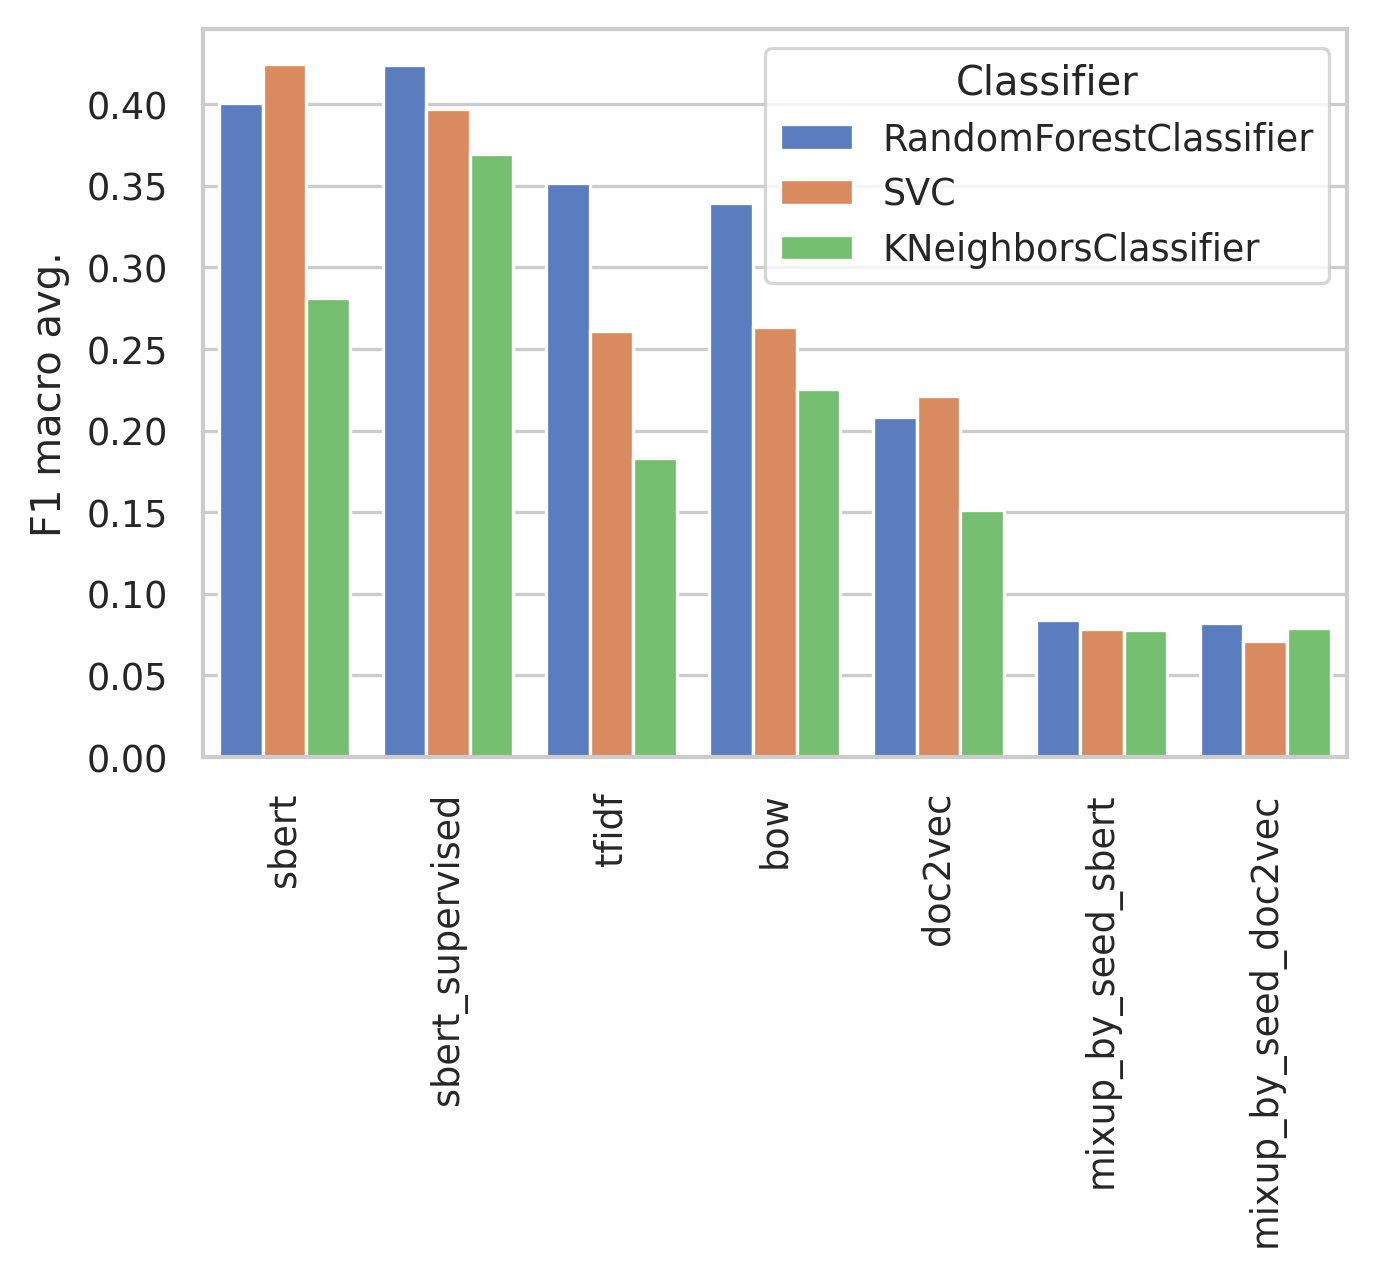
\includegraphics[width=0.5\textwidth]{figs/cls_gs_diff_embed_comparison.png}

  \caption{Grid search F1 macro averaged scores for transformation vectors.
  The reported scores of \Embed{sbert\_supervised} are the mean scores of all
  SBERT supervised embeddings.
  }\label{fig:cls_gs_diff_embed_comparison}

\end{figure}

Moreover the BOW embeddings surpassed \Embed{doc2vec} embedding,
proving that for prediction of transformation, lexical features are more
valuable than any information extracted by our trained Doc2vec model.

% TODO?: Should I mention the suprising performance of RandomForest on sparse
% embeddings?

In Figure~\ref{fig:cls_gs_diff_labels} we show the performance of best
classifiers per each label for the most performant dense and lexical
embeddings: \Embed{sbert} and \Embed{tfidf}. We can identify four
transformations as being well-predicted having around 0.80 f1-score. However
the powerful processing of SBERT offered significant advantage to pure lexical
information only for two of those: \Trans{past} and \Trans{future}. We see even
bigger difference for \Trans{opposite meaning}, even if it reached just 0.4
f1-score.

\begin{figure}[htp]
  \centering
  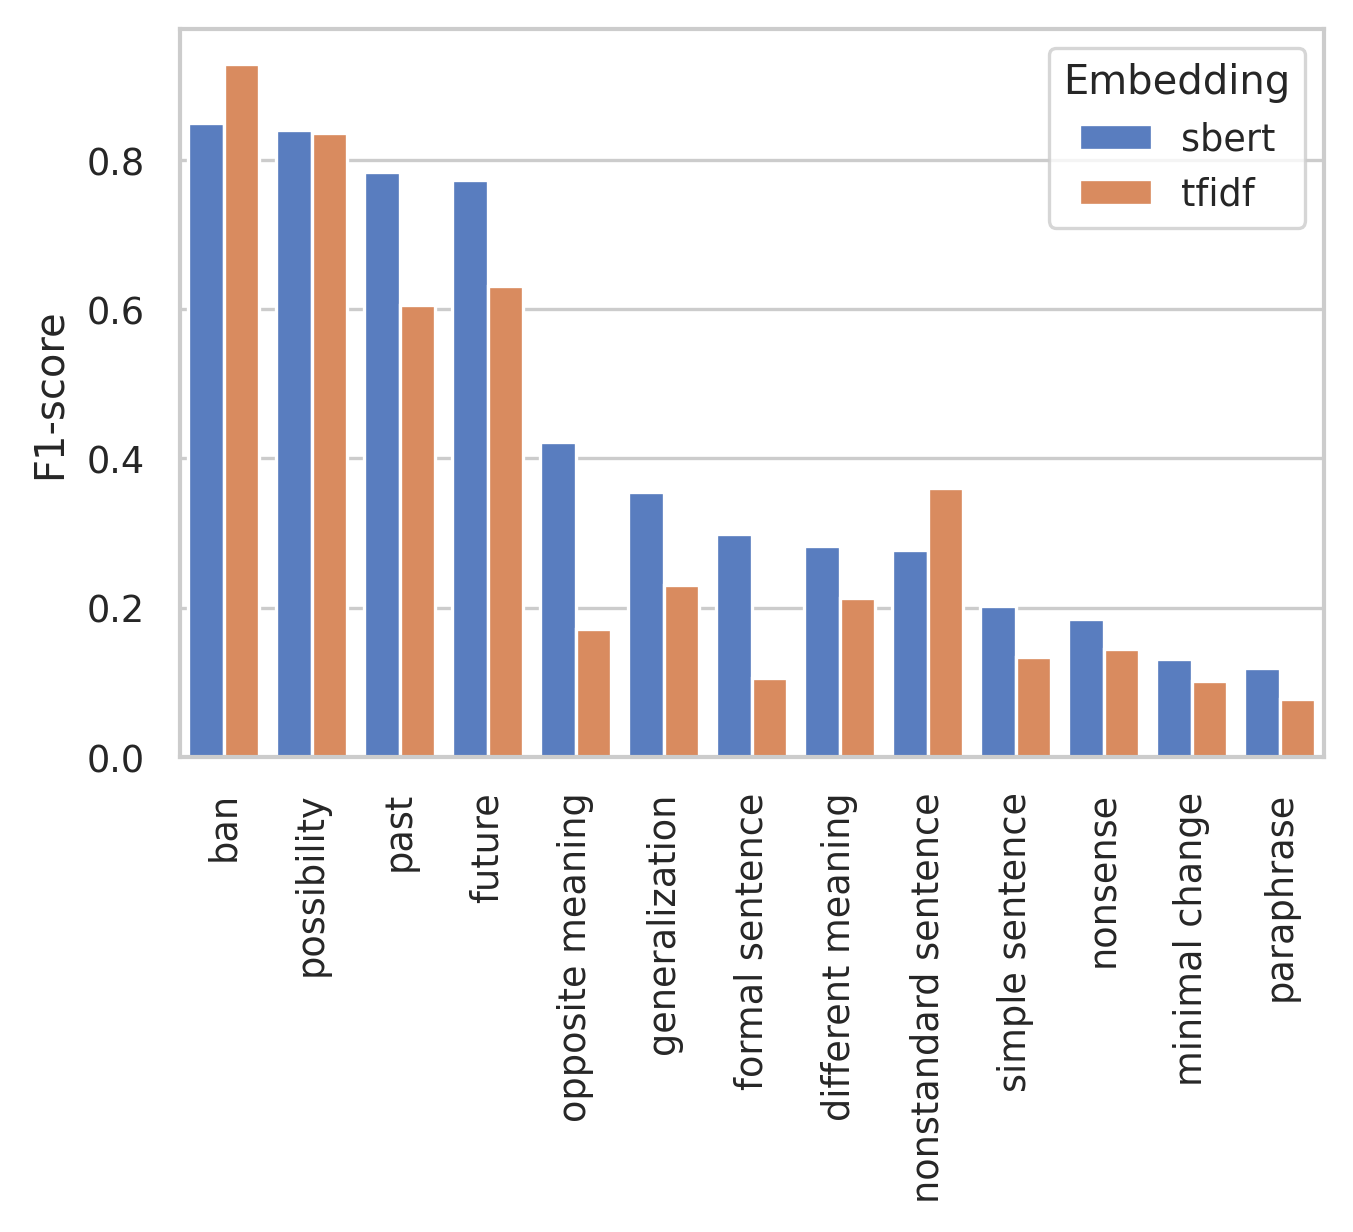
\includegraphics[width=0.5\textwidth]{./figs/cls_gs_diff_labels.png}

  \caption{F1 score of transformation vectors for each transformation of the
  best classifiers for given embedding.}\label{fig:cls_gs_diff_labels}

\end{figure}

In order to examine the most confused transformations we summed confusion
matrices of the top 3 most performant embeddings. The resulting matrix is shown
in Figure~\ref{fig:cls_gs_diff_conf_mat}. The most confused pairs of
transformations are \Trans{minimal change} with \Trans{different meaning} and
\Trans{nonsense} with \Trans{different meaning}, both in around 40\%.
Interestingly \Trans{paraphrase} gets recognised almost never, with
\Trans{simple sentence}, \Trans{formal sentence}, \Trans{nonsense} and
\Trans{minimal change} having accuracy bellow 20\%.

\begin{figure}[htp]
  \centering
  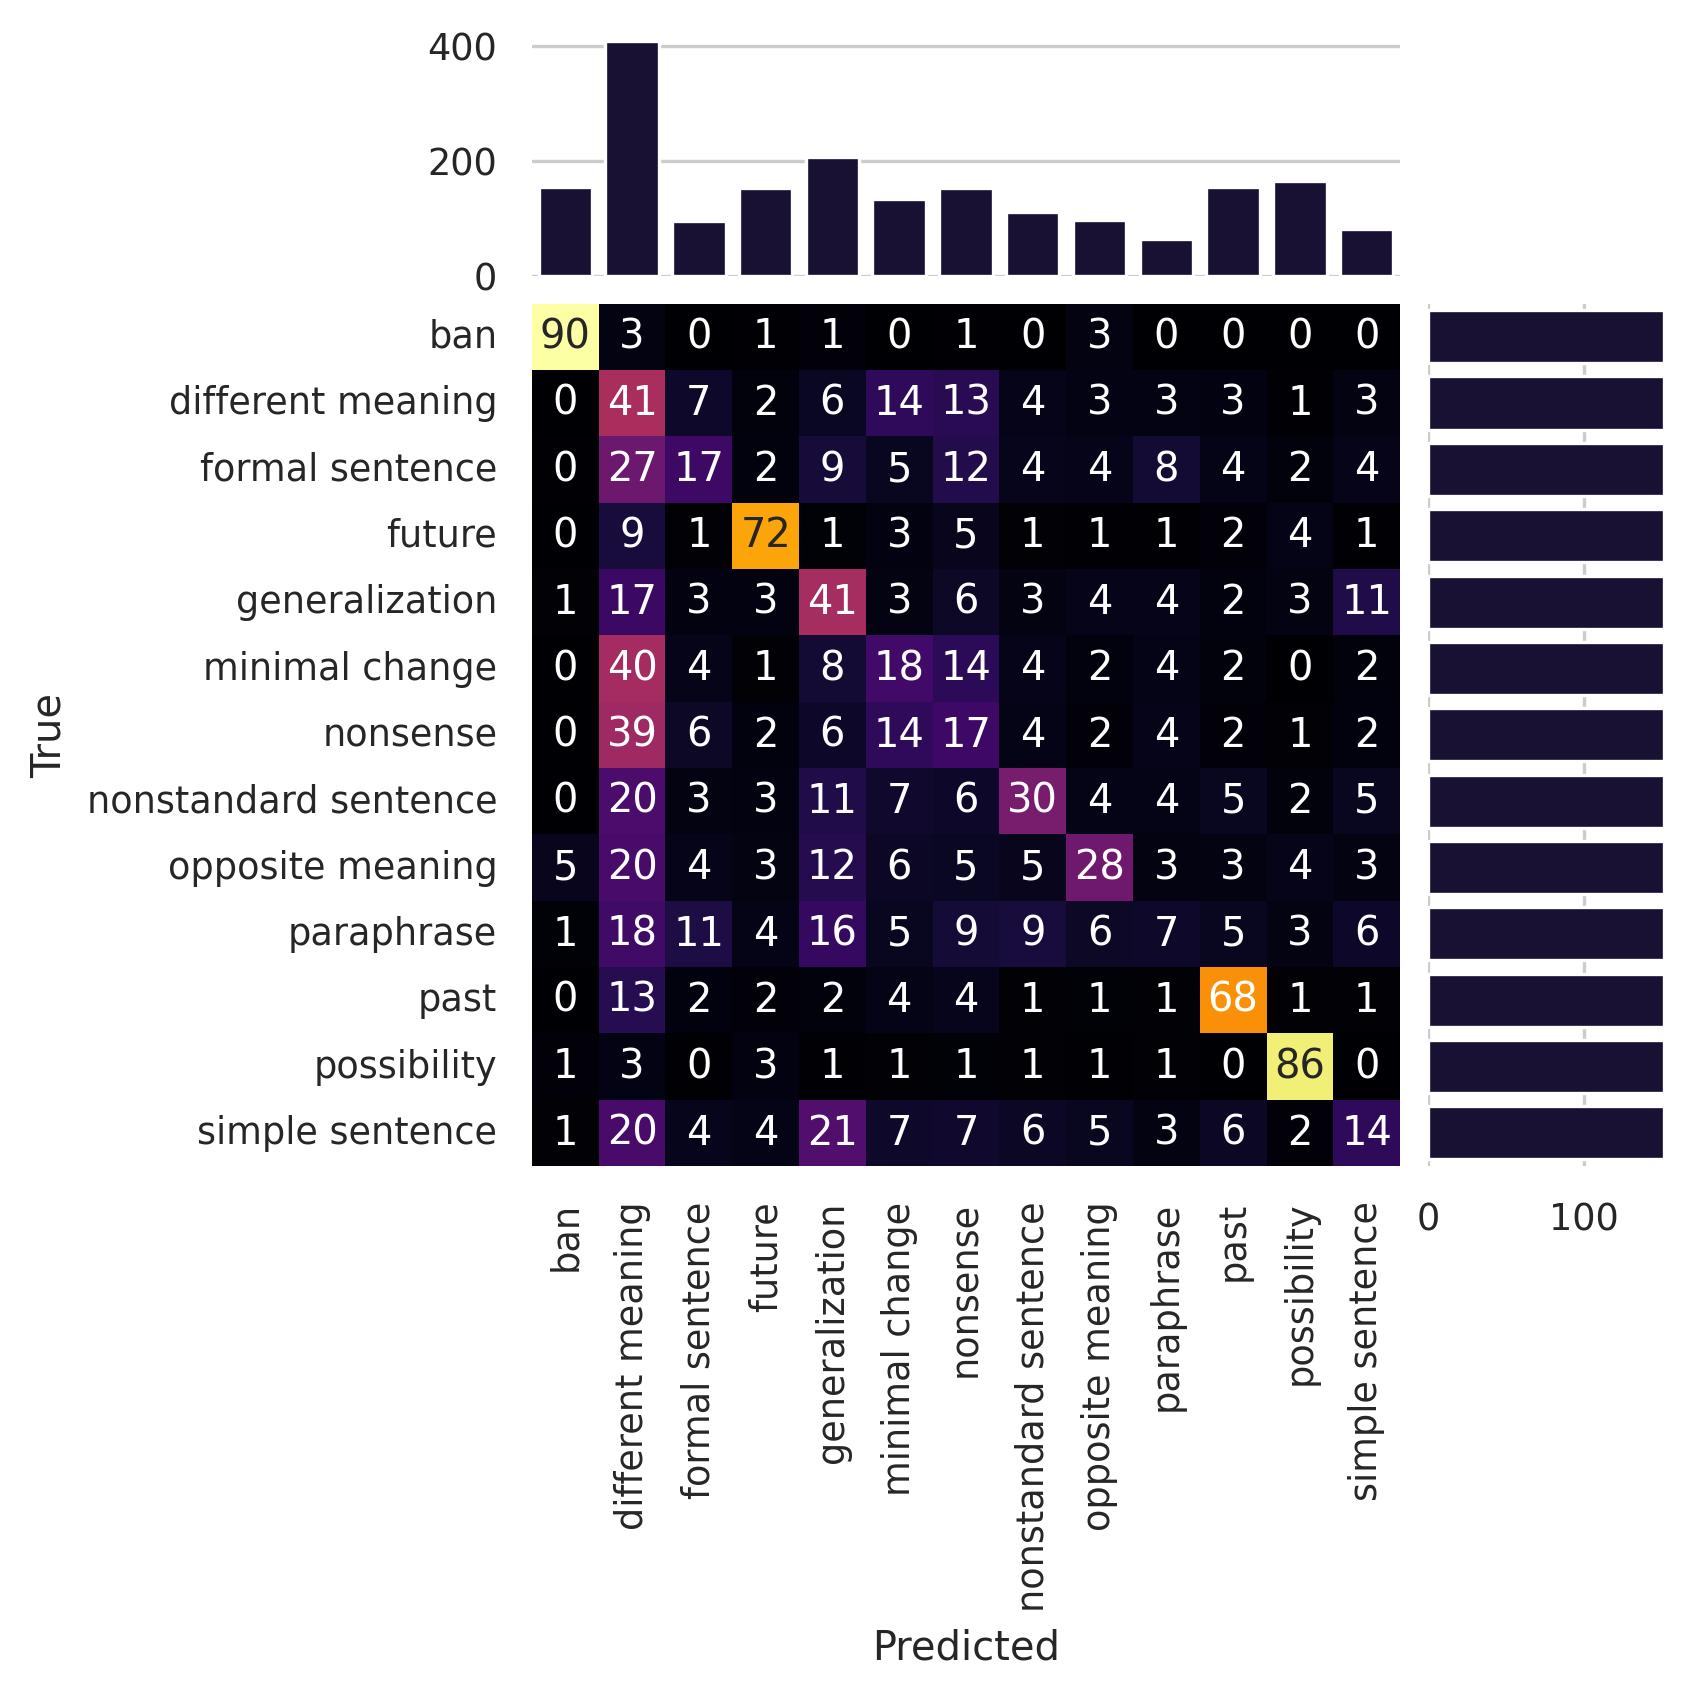
\includegraphics[width=0.5\textwidth]{./figs/cls_gs_diff_conf_mat.png}
  \caption{Summed confusion matrices of best classifiers for \Embed{sbert},
  \Embed{sbert\_supervised} and \Embed{tfidf} embeddings. The confusion matrix
  is row-normalized, whereas the displayed true and predicted distributions are
  not.}\label{fig:cls_gs_diff_conf_mat}
\end{figure}

\subsubsection{Classifying sentence embeddings}

Again, we report plotted grid search results in
Figure~\ref{fig:cls_gs_no_context_embed_comparison}. Comparing these results to
results for probing transformation vectors, we see large drop of performance for
\Embed{sbert} embedding --- almost by 50\%. This shows how much the classifiers
relied on the information contained in the embedding of seed sentence. This
drop is not as pronounced for \Embed{sbert\_supervised} embedding, because the
model producing them is optimized with precisely this type of
task.\footnote{For this reason, we avoid comparing \Embed{sbert\_supervised} to
other embeddings from this point onwards.} On the other hand, the BOW
embeddings performed almost as well, suggesting they were not really able to
take advantage of the information inside seed embeddings.

\begin{figure}[htp]
  \centering
  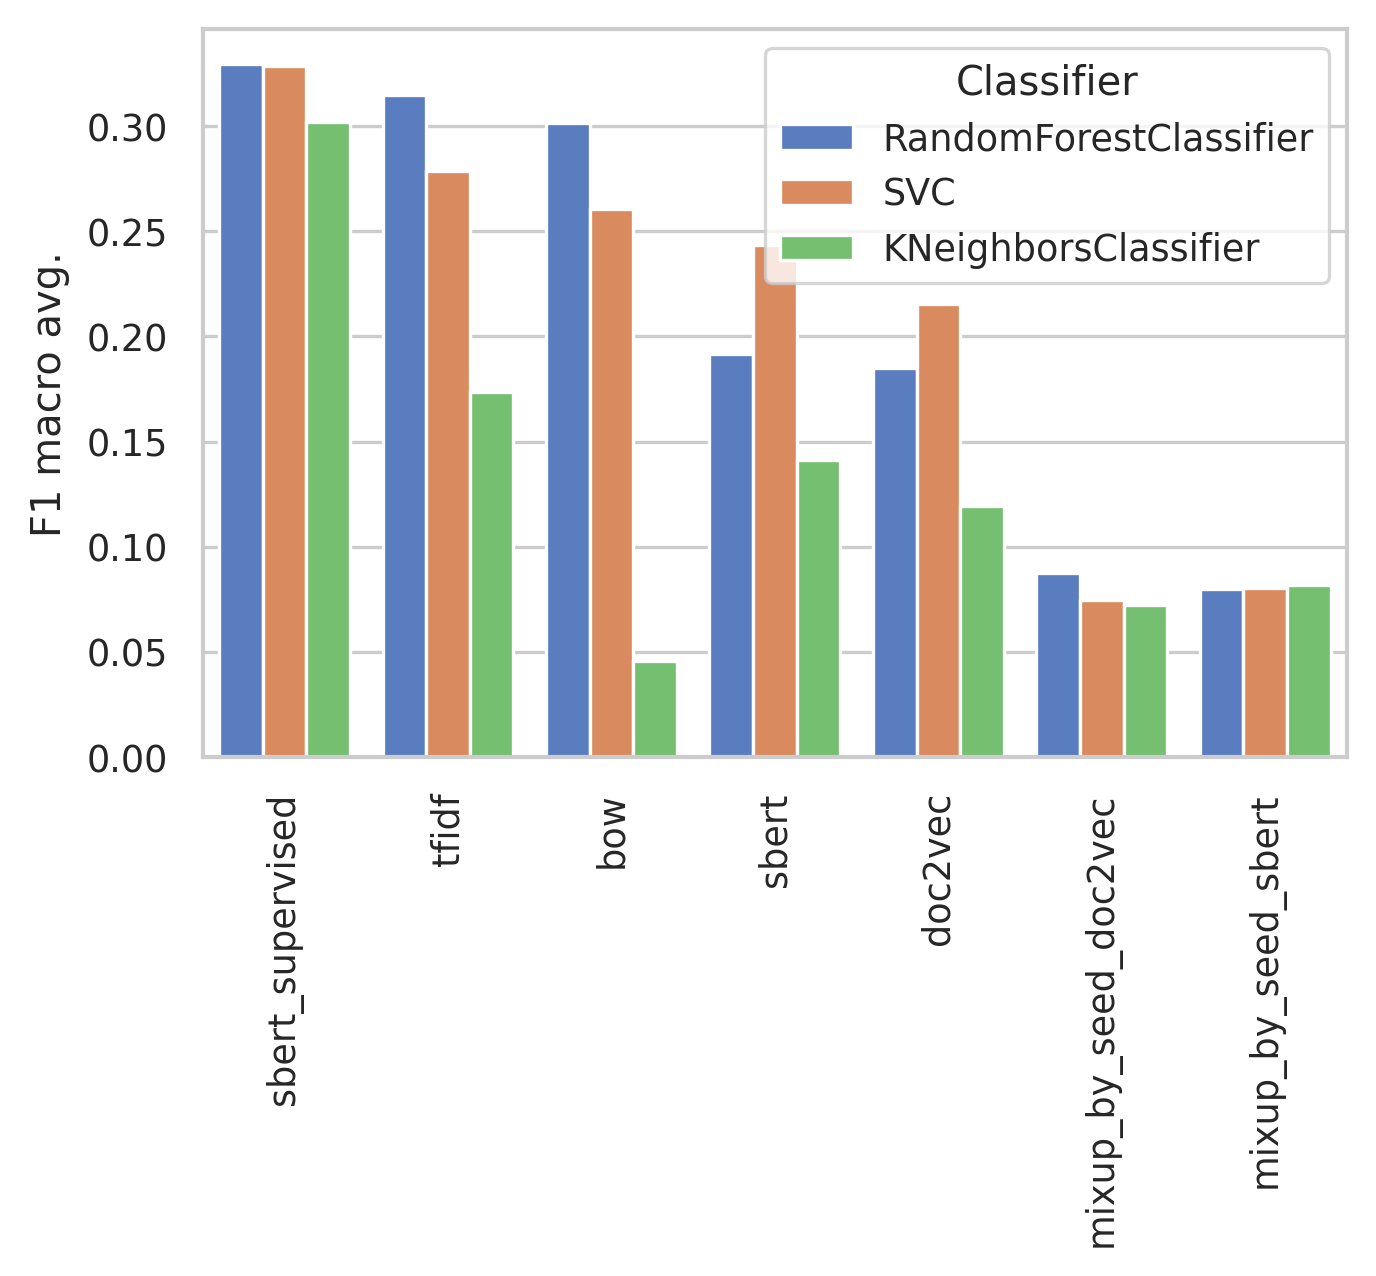
\includegraphics[width=0.5\textwidth]{./figs/cls_gs_no_context_embed_comparison.png}

  \caption{Grid search F1 macro averaged scores of sentence embeddings. The
  reported scores of \Embed{sbert\_supervised} are the mean scores
  of all SBERT supervised
  embeddings.}\label{fig:cls_gs_no_context_embed_comparison}

\end{figure}

In Figure~\ref{fig:cls_gs_no_context_labels} we compare performance of best
classifiers for \Embed{sbert} and \Embed{tfidf} embedding. Whereas the most
recognised transformations are the same as when classifying transformation
vectors, the classifiers performance significantly drops in all cases except
for the \Trans{ban} and the \Trans{possibility} transformations embedded with
TF-IDF. This suggests that \Trans{ban} and \Trans{possibility} transformations
can be easily identified from pure \emph{lexical} features and based on the
sentence embedding only. While SBERT fails to encode this information into its
embedding, it performs even better than TF-IDF when the embeddings of a
sentence and its corresponding seed sentence are put into one context. As can
be seen in Figure~\ref{fig:cls_gs_labels_context_diff}, this phenomena is
pronounced mainly for \Trans{different meaning} and \Trans{past}
transformations, where the inclusion of seed sentence's embedding on the input
is responsible for over 80\% and 60\% of F1 score of the classifier. Overall
SBERT's embeddings benefit from including the seed embedding to the input more
than TF-IDF vectors.

\begin{figure}[htp]
  \centering
  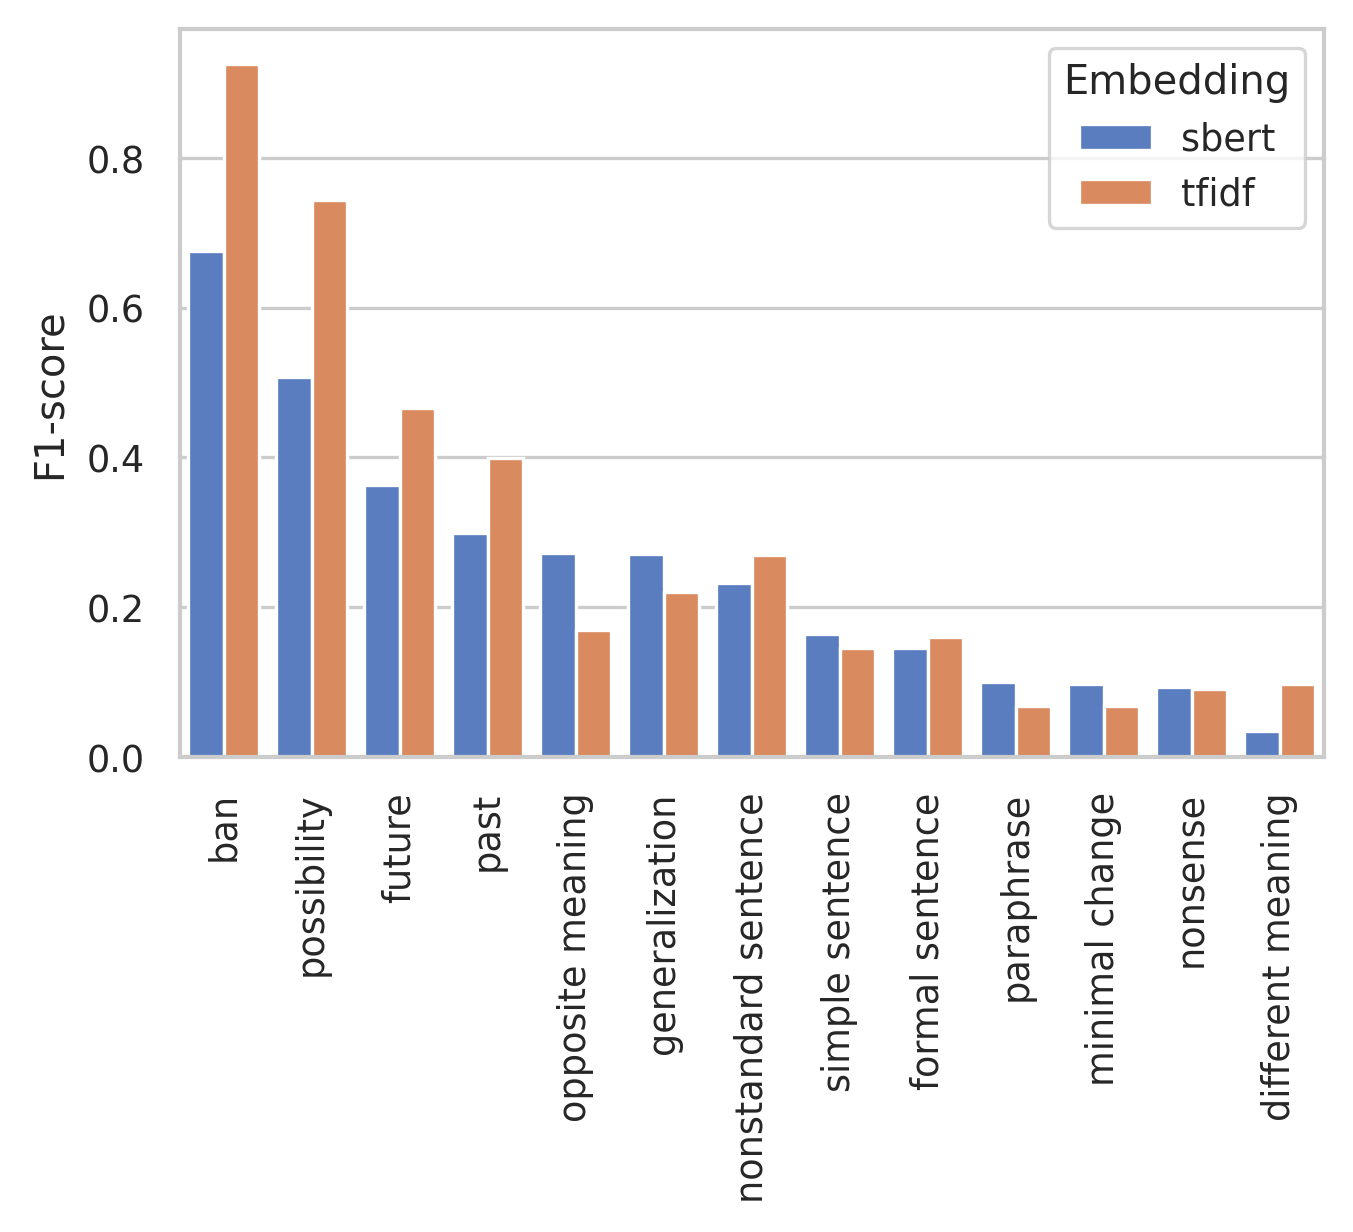
\includegraphics[width=0.5\textwidth]{figs/cls_gs_no_context_labels.png}

  \caption{F1 scores of sentence embeddings for each transformation of the best
  classifiers for given embedding.}\label{fig:cls_gs_no_context_labels}

\end{figure}

\begin{figure}[htp]
  \centering
  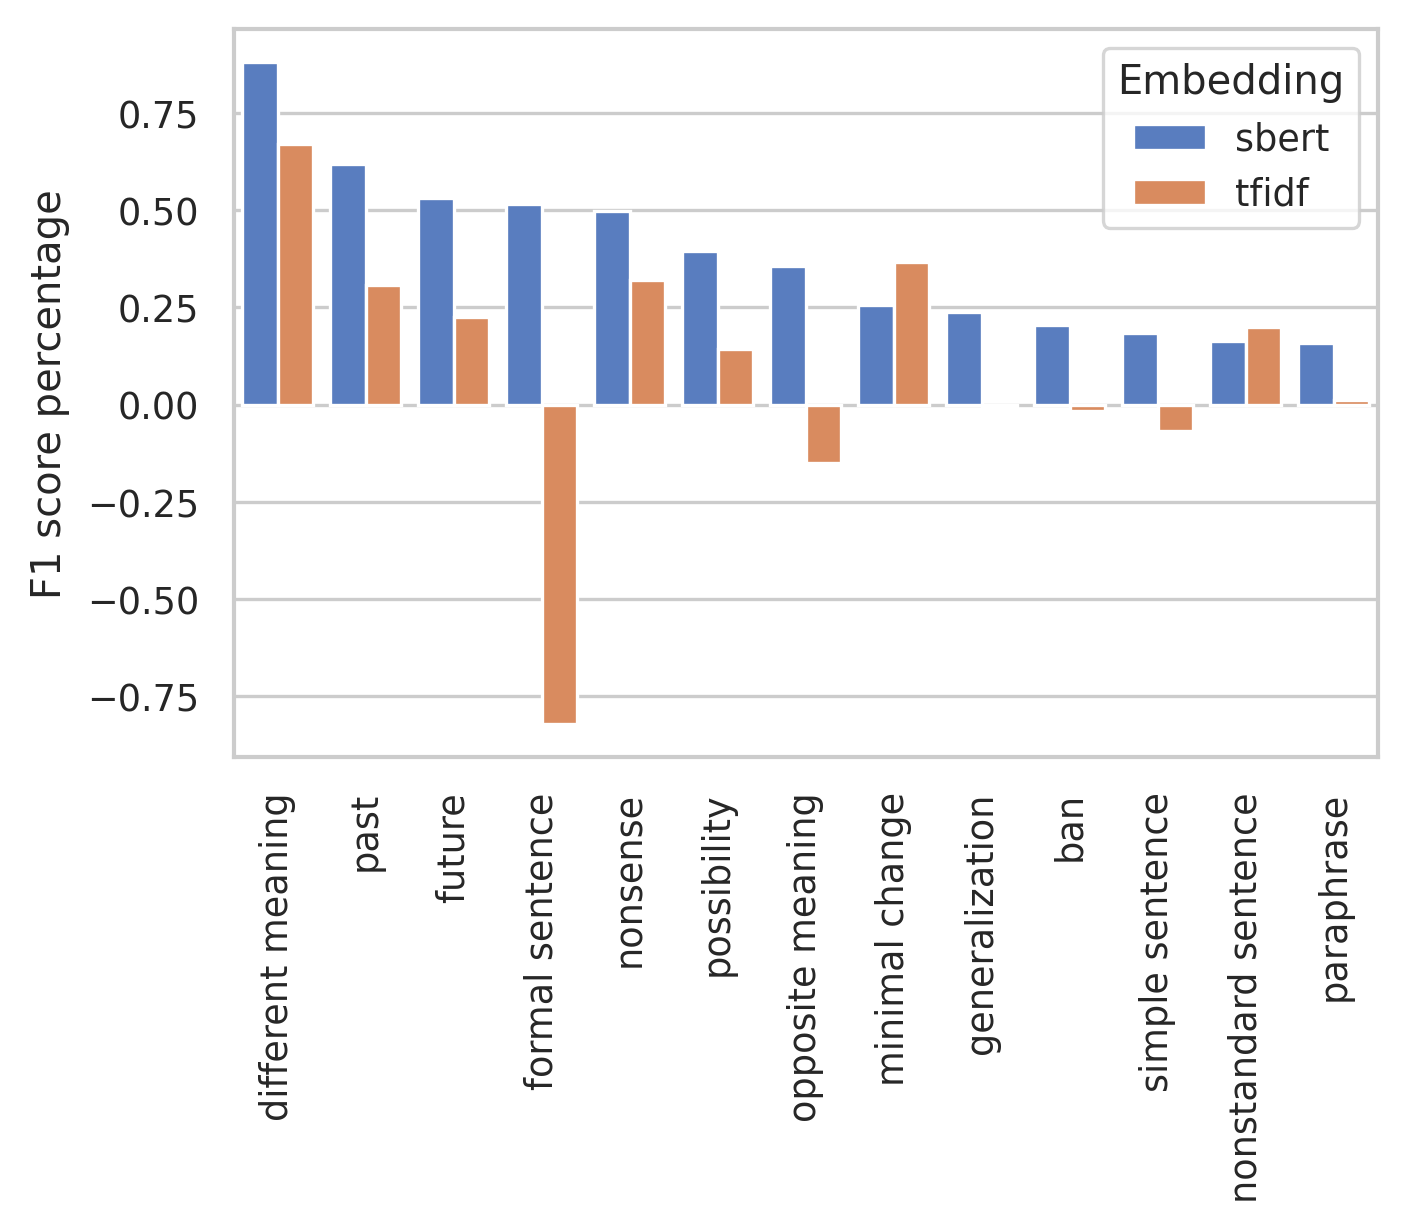
\includegraphics[width=0.5\textwidth]{figs/cls_gs_labels_context_diff.png}

  \caption{Drop in performance of best classifiers for given embedding going
  from transformation vector to sentence embedding classification. The drop is
  given as a percentage of score for transformation
  vectors.}\label{fig:cls_gs_labels_context_diff}.

\end{figure}

\subsection{Evaluating Sentence Embeddings with Gaussian Mixture}

This section presents an unsupervised approach for evaluating the separability
of sentence embeddings. We measure label separability pairwisely using a
Gaussian Mixture model and calculate the F-score of the unsupervised clustered
labels with the true labels.

The Gaussian Mixture model is a probabilistic model that assumes that each
cluster follows a Gaussian (or normal) distribution and estimates the weight of
the density function for each cluster~\cite{reynolds2009gaussian,5298967}. We
assume that the sentence vectors of two distinct classes should achieve high
accuracy with Gaussian Mixture if they are displayed in a Gaussian distribution
in space and are separable from each other.

However, there is a potential limitation to using this method. The separability
and accuracy score may be underestimated if two clusters are not normally
distributed, as illustrated in Figure~\ref{fig:cirle}.


\begin{figure}[htp]
    \centering
    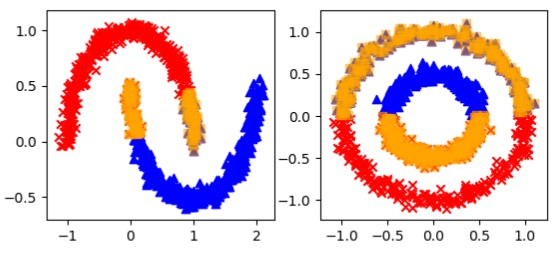
\includegraphics[scale=0.4]{figs/Circle.jpg}
    \caption{Cases that Gaussian Mixture Underestimate the Separability of Two
    Clusters}\label{fig:cirle}
\end{figure}


Our evaluation results show that out of 78 pairs of derivation classes, 7 pairs
achieved an accuracy score above 90\%, 24 pairs above 80\%, and 47 pairs above
60\%, as depicted in Figure~\ref{fig:GM}.

In particular, the class `ban' demonstrates good separability with many other
classes, achieving an accuracy score of 0.982 with `past', 0.980 with `formal
sentence', 0.942 with `minimal change', and 0.937 with `future', among other
pairs.

Additionally, our evaluation results reveal that tenses are generally
well-separated, with an accuracy score of 0.90 for `past' and future' classes,
and an accuracy score of 0.924 for `simple sentence' and `future' classes.

\begin{figure}[htp]
    \centering
    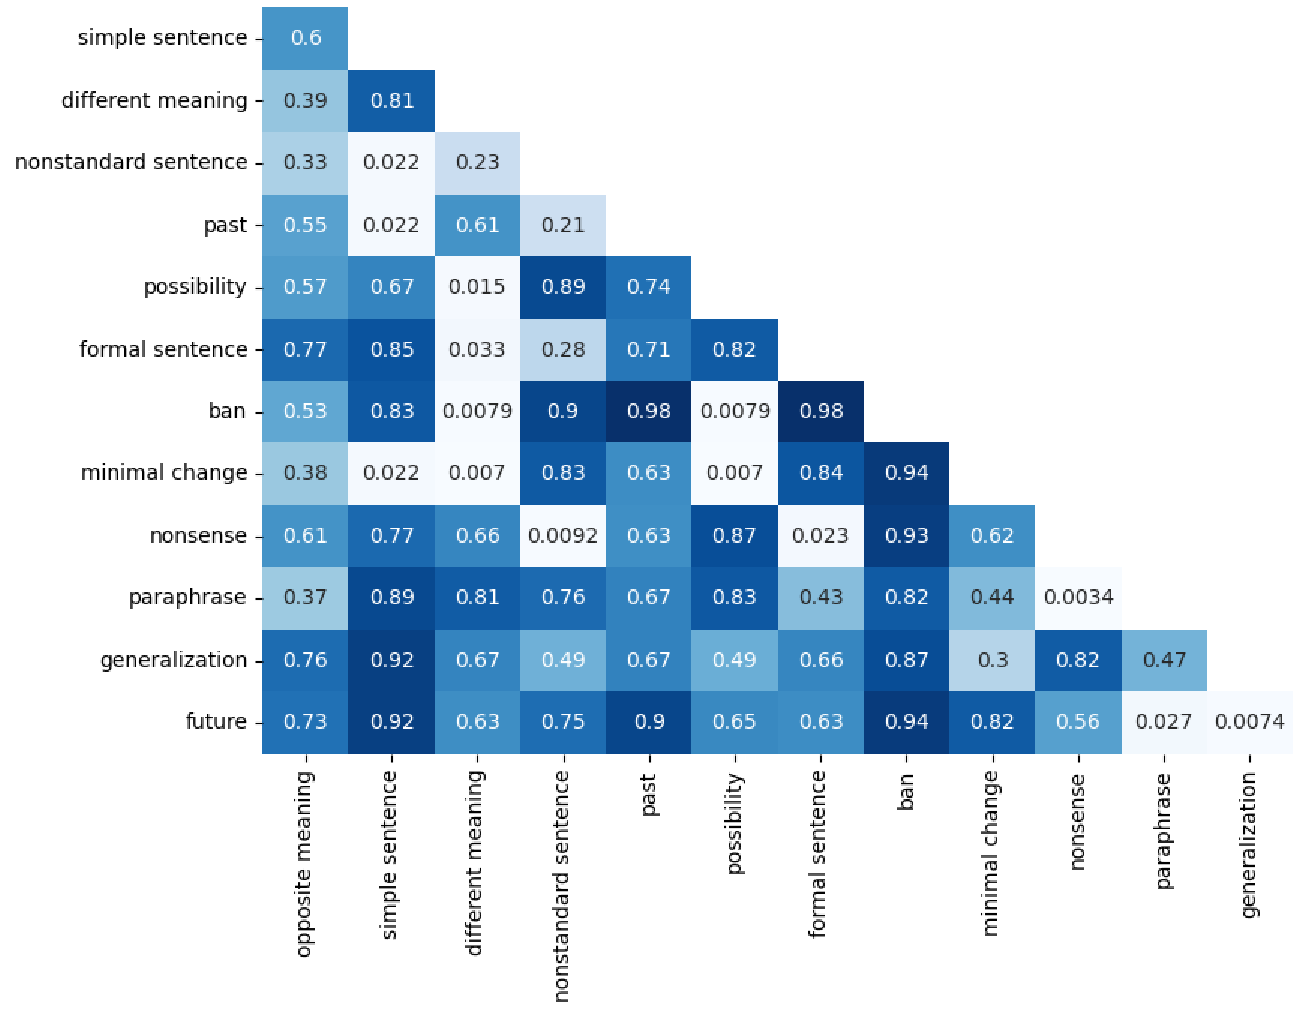
\includegraphics[scale=0.4]{figs/GM.png}
    \caption{Accuracy of Measured Separability with Gaussian
    Mixture}\label{fig:GM}
\end{figure}





% \subsection{SBERT as a classifier}
% This section shows whether the sentence embeddings trained on our models can
% serve as a classifier and separate sentences in terms of labels.

% For each derivation sentence, we compute the distance from its seed. The
% resulting vector. It is assumed that a certain type of derivation from a seed
% shares some similarities. A good classifier is assumed to group the same
% derivation types. For example, (sentence vector - seed vector)sentences with
% future tense are supposed to group together.
% visualize the distance vecotors 

% reduced dimension PCA


% Sentence embeddings trained with SBERT can serve as classifier for some
% labels. For instance, the embeddings can separate 'future','past' and 'simple
% sentence' as in Figure X
% However, it does not work for the rest of groups: 

% \subsection{Degree of Transformation}

% Whether the degree of transformation can be characterized by SBERT sentence
% embeddings. It shows the generalization group achieved most correlation. The
% more generalized sentences are further from seed sentence. While less
% generalized sentences (sentence meaning closer to seed sentences) has shorter
% distance to seed sentences

\section{Conclusion}

% Summarize our results. Put them to context?

\bibliography{bibliography}
\bibliographystyle{acl_natbib}

\clearpage
\appendix
\section{SBERT embeddings}\label{appendix:sbert_embeddings}

For SBERT implementation we used the
\texttt{sentence\_transformers}\footnote{\url{https://www.sbert.net/}} python
library.

To produce sentence embeddings with SBERT, we chose pretrained model referred
to as `\textit{paraphrase-multilingual-MiniLM-L12-v2}'. It offers relatively
good scores for its size.

For the supervised SBERT sentence embeddings we list the hyperparameters used
in Table~\ref{tab:sbert_supervised_hparams}. Note that due to the small size of
training data, the model overfitted quickly. We therefore could afford to train
only for 4 epochs.

\begin{table}[htp]
  \centering
  \begin{tabular}{l c}
    \toprule
    Hyperparameter & Value\\
    \midrule
    epochs & 4 \\
    batch size & 8 \\
    warmup schedule & linear \\
    warmup steps & 10000 \\
    optimizer & AdamW \\
    weight decay & 0.1 \\
    learning rate & 2e-5 \\
    \bottomrule
  \end{tabular}

  \caption{Hyperparameters used to train SBERT for supervised
  embeddings}\label{tab:sbert_supervised_hparams}

\end{table}

\section{Probing method in detail}\label{appendix:probing_method}

For probing tasks whose results we described in
Section~\ref{sec:probing_results}, we used
\texttt{scikit-learn}\footnote{\url{https://scikit-learn.org/stable/}} python
package.

The grid searched parameters and classifiers are presented in
Table~\ref{tab:cls_gs_all_params}. We used cross-validated grid search, where
the performence of a set of parameters is evaluated using cross validation. For
all cross validations (both within and outside of grid search) we used
\texttt{StratifiedGroupKFold}, where seed identifiers were used as groups. This
caused the folds to be stratified as well as sharing as few common seed
sentences as possible.

\begin{table*}[htp]
  \centering

  \begin{tabular}{l l l}
    \toprule
    Classifier & Hyperparameter & Values searched \\
    \midrule
    \multirow{3}{13em}{\Cls{RandomForestClassifier}}
    & \texttt{n\_estimators} & 50, 100, 200 \\
    & \texttt{max\_depth} & 2, 5, 25, None \\
    & \texttt{min\_samples\_split} & 2, 10, 20 \\
    \midrule
    \multirow{2}{13em}{\Cls{SVC}*}
    & \texttt{kernel} & rbf, linear \\
    & \texttt{gamma} & auto, scale\\
    \midrule
    \multirow{2}{13em}{\Cls{KNeighboursClassifier}*}
    & \texttt{n\_neighbours} & 3, 5, 10\\
    & \texttt{weights} & uniform, distance\\
    \bottomrule
  \end{tabular}

  \caption{Classifiers and hyperparameters grid search for probe tasks. All are
  named equally as in the \texttt{scikit-learn} python package. *Embeddings
  were first scaled to have zero mean and unit
  variance.}\label{tab:cls_gs_all_params}

\end{table*}

We report the best performing set of parameters for each classifier in
Tables~\ref{tab:cls_gs_best_params_SVC},~\ref{tab:cls_gs_best_params_RandomForestClassifier}~and~\ref{tab:cls_gs_best_params_KNeighborsClassifier}

\begin{table*}[htp]
  \centering
  \begin{tabular}{lcccc}
\toprule
&  & \texttt{gamma} & \texttt{kernel} \\
Context & Embedding &  &  \\
\midrule
\multirow[c]{2}{*}{diff} & \Embed{doc2vec} & auto & rbf \\
& \Embed{sbert} & auto & rbf \\
\noalign{\smallskip}
\cline{1-4}
\noalign{\smallskip}
\multirow[c]{4}{*}{no-context} & \Embed{doc2vec} & auto & rbf \\
& \Embed{sbert} & auto & rbf \\
& \Embed{sbert\_supervised\_0} & auto & rbf \\
& \Embed{sbert\_supervised\_2} & auto & rbf \\
\bottomrule
\end{tabular}


  \caption{Best parameters for \Cls{SVC}
  classifier.}\label{tab:cls_gs_best_params_SVC}

\end{table*}

\begin{table*}[htp]
  \centering
  \begin{tabular}{lccccc}
\toprule
&  & \texttt{max\_depth} & \texttt{min\_samples\_split} & \texttt{n\_estimators} \\
Context & Embedding &  &  &  \\
\midrule
\multirow[c]{9}{*}{diff} & \Embed{bow} & 25 & 20 & 200 \\
& \Embed{mixup\_by\_seed\_doc2vec} & None & 5 & 200 \\
& \Embed{mixup\_by\_seed\_sbert} & 25 & 5 & 200 \\
& \Embed{sbert\_supervised\_0} & None & 5 & 200 \\
& \Embed{sbert\_supervised\_1} & None & 5 & 200 \\
& \Embed{sbert\_supervised\_2} & 25 & 10 & 200 \\
& \Embed{sbert\_supervised\_3} & None & 5 & 200 \\
& \Embed{sbert\_supervised\_4} & None & 10 & 100 \\
& \Embed{tfidf} & None & 20 & 200 \\
\noalign{\smallskip}
\cline{1-5}
\noalign{\smallskip}
\multirow[c]{6}{*}{no-context} & \Embed{bow} & 25 & 10 & 200 \\
& \Embed{mixup\_by\_seed\_doc2vec} & None & 20 & 50 \\
& \Embed{sbert\_supervised\_1} & 25 & 10 & 50 \\
& \Embed{sbert\_supervised\_3} & 25 & 10 & 100 \\
& \Embed{sbert\_supervised\_4} & 25 & 5 & 50 \\
& \Embed{tfidf} & 25 & 10 & 200 \\
\bottomrule
\end{tabular}


  \caption{Best parameters for \Cls{RandomForestClassifier}
  classifier.}\label{tab:cls_gs_best_params_RandomForestClassifier}

\end{table*}

\begin{table*}[htp]
  \centering
  \begin{tabular}{lcccc}
\toprule
&  & \texttt{n\_neighbors} & \texttt{weights} \\
Context & Embedding &  &  \\
\midrule
no-context & \Embed{mixup\_by\_seed\_sbert} & 5 & distance \\
\bottomrule
\end{tabular}


  \caption{Best parameters for \Cls{KNeighboursClassifier}
  classifier.}\label{tab:cls_gs_best_params_KNeighborsClassifier}

\end{table*}

% chosen parameters



\end{document}
